\pdfoutput=1
\begin{figure}[tb!]
    \centering
    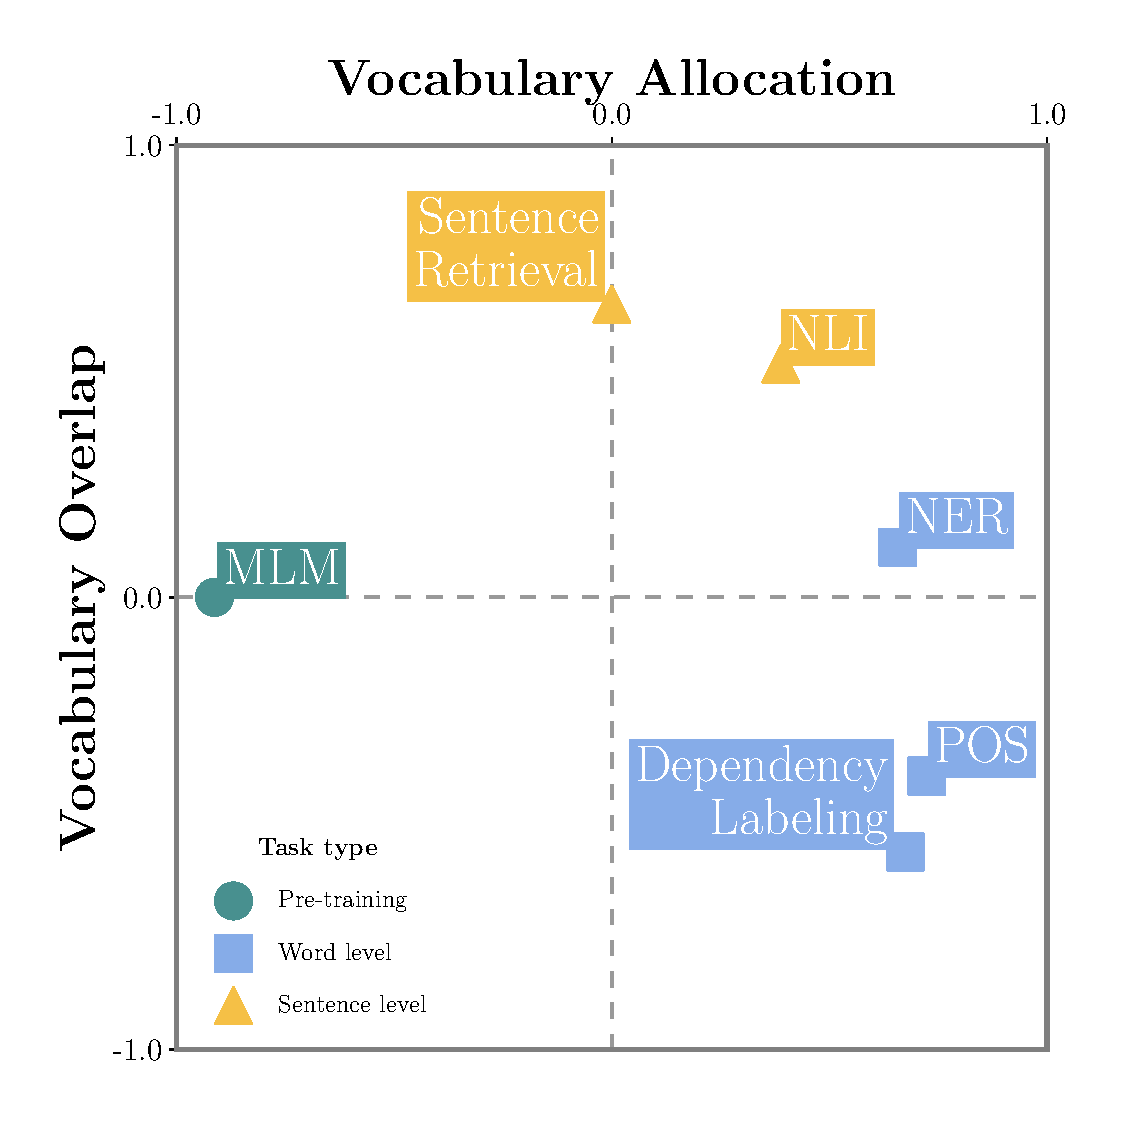
\includegraphics[width=\linewidth]{figures/Schwartz_camread_.pdf}

    \caption{Mapping the impact of \va~and \vo~on language model performance. The location of points corresponds to Spearmnan's correlation between vocabulary measures and the task score (see the details in Tables~\ref{tab:corr_in_lang_20l}~and~\ref{tab:corr_x_lang_6l}). High \vo~benefits NER and sentence-level tasks (NLI, sentence retrieval) and hinders POS and dependency labeling performance. High \va~improves word-level tasks but leads to a decrease in masked language modeling scores. 
    %The location of the points is defined by the Spearman correlation between the task score and \va~measure (CPT) and \vo~measure (-JSD). For details see Tables~\ref{tab:corr_in_lang_20l}~and~\ref{tab:corr_x_lang_6l}.
    Masked language modeling is measured only in language. Thus it's unaffected by \vo. Analogically, sentence retrieval is solely cross-lingual and unaffected by \va.}
    \label{fig:schwartz}
\end{figure}